\section{Algoritmos para lenguajes regulares}

\subsection{Evaluación de expresiones regulares}

\paragraph{Expresiones regulares en la práctica.} El lenguaje para definir expresiones regulares en la práctica se conoce como \textbf{RegEx} (o RexExp). Las sintaxis más usadas para definir \textbf{RegEx} son:
\begin{enumerate}
    \item POSIX (Portable Operating System Interface for uniX).
    \item Perl (PCRE $=$ Perl Compatible Regular Expressions).
\end{enumerate}

\begin{table}[H]
    \centering
    \begin{tabular}{lcc}
                          & RegEx                                     & Teoría                                                       \\
        \hline
        Carácter          & $\texttt{a}$                              & $\mathrm{a}$                                                 \\
        Escape            & $\backslash+$                             & $-$                                                          \\
        Cualquiera        & $\cdot$                                   & $\Sigma$                                                     \\
        Clase             & {$\texttt{[abc]}$}                        & $(a+b+c)$                                                    \\
        Clase consecutivo & {$\texttt{[a-zA-Z]}$}                     & $(a+\cdots+z+A+\cdots+Z)$                                    \\
        Clase exclusivo   & {$\texttt{[} \texttt{\^{}}\texttt{0-9]}$} & $\left(++_{a \in \Sigma-\{0, \ldots, 9\}} \mathrm{a}\right)$ \\
        Alternación       & $\texttt{cat} \mid \texttt{dog}$          & $\mathrm{cat}+\mathrm{dog}$                                  \\
        0 o 1             & $\texttt{R} ?$                            & $R^?$                                                        \\
        1 o más           & $\texttt{R}+$                             & $R^{+}$                                                      \\
        0 o más           & $\texttt{R} *$                            & $R^*$                                                        \\
        entre $n$ y $m$   & $\texttt{R}\{\texttt{n}, \texttt{m}\}$    & $R^n(R+\epsilon)^{m-n}$                                      \\
        Backreference     & $(\mathrm{R}) \backslash 1$               & $?$                                                          \\
        $\ldots$          & $\cdots$                                  & $\cdots$
    \end{tabular}
\end{table}

\paragraph{¿Cómo evaluamos una expresión regular?} Tenemos el siguiente problema:
\begin{table}[H]
    \centering
    \begin{tabular}{ll}
        $\texttt{PROBLEMA:}$ & Evaluación de expresiones regulares              \\
        $\texttt{INPUT:}$    & una expresión regular $R$                        \\
                             & un documento $w$                                 \\
        $\texttt{OUTPUT:}$   & $\texttt{TRUE}$ si, y sólo si, $w \in \ca{L}(R)$
    \end{tabular}
\end{table}

Donde el tamaño del input está dado por:
\begin{itemize}
    \item $|R|:=$ número de letras y operadores.
    \item $|w|:=$ largo del documento.
\end{itemize}

Buscamos un algoritmo polinomial en $\lvert R \rvert$ y $\lvert w\rvert$. Algo a notar es que $\lvert R\rvert <{}<\lvert w \rvert$:
\begin{itemize}
    \item $|R|$ puede ser del orden \textbf{decenas} operadores ($\sim$ 1 KB).
    \item $|w|$ puede ser del orden de \textbf{miles a millones} de símbolos ($\sim$ 100MB).
\end{itemize}

\paragraph{Análisis de tiempo diferenciado.} Tenemos dos tipos:
\begin{itemize}
    \item \textbf{Combined complexity:} expresión y documento son parte del input.
    \item \textbf{Data complexity:} solo documento es parte del input (tamaño de expresión es considerada una constante).
\end{itemize}

Buscamos algoritmos que sean \textbf{lineales en data complexity} y ojalá \textbf{polinomiales en combined complexity}. \medbreak

Volviendo a nuestro problema:
\begin{table}[H]
    \centering
    \begin{tabular}{ll}
        $\texttt{PROBLEMA:}$ & Evaluación de expresiones regulares              \\
        $\texttt{INPUT:}$    & una expresión regular $R$                        \\
                             & un documento $w$                                 \\
        $\texttt{OUTPUT:}$   & $\texttt{TRUE}$ si, y sólo si, $w \in \ca{L}(R)$
    \end{tabular}
\end{table}

Los pasos que podemos seguir para resolverlo son:
\begin{enumerate}
    \item Convertimos $R$ a un $\epsilon$-NFA $\ca{A}_R$.
    \item Verificamos si $w \in \ca{L}(\ca{A}_R)$.
\end{enumerate}
Ahora, el tamaño del input es:
\begin{itemize}
    \item $|w|:=$ largo del documento.
    \item $|\ca{A}|:= |Q| + |\Delta|$.
\end{itemize}

Hay varias soluciones para resolver nuestro problema, que iremos enumerado a continuación.

\paragraph{Solución 1: Backtracking.} Esta solución es la que usa la mayoría de los motores de RegEx en la práctica. Se puede hacer una prueba en \url{https://regexr.com/}.

\paragraph{Solución 2: DFA.} Para un DFA $\ca{A} = (Q,\Sigma,\delta, q_0, F)$ y una palabra $w = a_1 \ldots a_n$.
\vspace{-8pt}
\begin{algorithm}[hbt!]
    % \caption*{An algorithm with caption}\label{alg:two}
    \setstretch{1.25}
    \DontPrintSemicolon
    \SetKwFunction{FevalDFA}{eval-DFA}
    \SetKwProg{Fn}{Function}{:}{}
    \SetKw{Check}{check}
    \Fn{\FevalDFA{$\ca{A}$, $w$}}{
        $q := q_0$

        \For{$i=1$ \KwTo $n$}{
            $q := \delta(q,a_i)$
        }

        \Return{\Check $(q \in F)$}
    }
\end{algorithm}
\vspace{-8pt}
\paragraph{Solución 3: NFA determinización.} Para un NFA $\ca{A} = (Q,\Sigma,\Delta, I, F)$ y una palabra $w = a_1 \ldots a_n$.
\vspace{-8pt}
\begin{algorithm}[hbt!]
    % \caption*{An algorithm with caption}\label{alg:two}
    \setstretch{1.25}
    \DontPrintSemicolon
    \SetKwFunction{FevalNFA}{eval-NFA}
    \SetKwFunction{FevalDFA}{eval-DFA}
    \SetKwProg{Fn}{Function}{:}{}
    \Fn{\FevalNFA{$\ca{A}$, $w$}}{
    $\ca{A}^{\text{det}} := \texttt{NFAtoDFA}(\ca{A})$

    \Return{\FevalDFA{$\ca{A}^{\text{det}},w$}}
    }
\end{algorithm}

¿Es necesario construir la determinización completa? La respuesta es que no. Recordemos que es la determinización. Para un autómata no-determinista $\ca{A} = (Q,\Sigma,\Delta,I,F)$, definimos el autómata determinista (\textbf{determinización} de $\ca{A}$):
\alignformula{
\ca{A}^{\text{det}} = (2^Q,\Sigma,\delta^{\text{det}},q_0^\text{det},F^\text{det})
}
\begin{itemize}
    \item $2^Q = \{S \mid S\subseteq Q\}$ es el conjunto potencia de $Q$.
    \item $q_0^\text{det} = I$.
    \item $\delta^\text{det}: 2^Q \times \Sigma \to 2^Q$ tal que:
          $$
              \delta^\text{det}(S,a) = \{q \in Q \mid \exists p \in S.\ (p,a,q) \in \Delta\}
          $$
    \item $F^\text{det} = \{S \in 2^Q \mid S \cap F \neq \varnothing\}$, es decir, todos los conjuntos que tengan al menos un estado final.
\end{itemize}

\paragraph{Solución 4: NFA \textit{on-the-fly}.} Fijémonos en la función de transición $\delta^\text{det}: 2^Q \times \Sigma \to 2^Q$ tal que:
$$
    \delta^\text{det}(S,a) = \{q \in Q \mid \exists p \in S.\ (p,a,q) \in \Delta\}
$$

La estrategia \textit{on-the-fly} corresponde a:
\begin{enumerate}
    \item Mantenemos un conjunto $S$ de estados actuales.
    \item Por cada nueva letra $a$, calculamos el conjunto $\delta^{\text{det}}(S,a)$.
\end{enumerate}
\fig{img/cap3/nfaonthefly.png}{0.2}{Ejemplo de NFa \textit{on-the-fly}}

Definimos el algoritmo para un NFA $\ca{A}=(Q,\Sigma,\Delta,I,F)$ y una palabra $w = a_1 \ldots a_n$ como:
\vspace{-8pt}
\begin{algorithm}[hbt!]
    % \caption*{An algorithm with caption}\label{alg:two}
    \setstretch{1.25}
    \DontPrintSemicolon
    \SetKwFunction{FevalNFAonthefly}{eval-NFAonthefly}
    \SetKwProg{Fn}{Function}{:}{}
    \SetKw{Check}{check}
    \Fn{\FevalNFAonthefly{$\ca{A}$, $w$}}{
        $S := I$

        \For{$i = 1$ \KwTo $n$}{
            $S_\text{old} := S$

            $S := \varnothing$

            \ForEach{$p \in S_\text{old}$}{
                $S := S \cup \{q \mid (p, a_i,q) \in \Delta\}$
            }
        }

        \Return{\Check $(S \cap F \neq \varnothing)$}
    }
\end{algorithm}

\paragraph{Resumen y complejidades.} Para un autómata $\ca{A}$ y una palabra $w = a_1 \ldots a_n$ tenemos que:

\begin{table}[H]
    \centering
    \begin{tabular}{lc}
                                           & Tiempo                                        \\
        \hline
        Backtracking                       & $\mathcal{O}\left(|\mathcal{A}|^{|w|}\right)$ \\
        DFA                                & $\mathcal{O}(|\mathcal{A}|+|w|)$              \\
        NFA                                & $\mathcal{O}\left(2^{|Q|}+|w|\right)$         \\
        $\epsilon$-NFA \textit{on-the-fly} & $\mathcal{O}(|\mathcal{A}| \cdot|w|)$
    \end{tabular}
\end{table}


\subsection{Transductores}
\fig{img/cap3/transductor.png}{0.2}{Representación de un transductor}

\paragraph{Definición.} Un transductor (en inglés, \textit{transducer}) es una tupla:
\alignformula{
    \ca{T} = (Q,\Sigma,\Omega,\Delta,I,F)
}
\begin{itemize}
    \item $Q$ es un conjunto finito de estados.
    \item $\Sigma$ es el alfabeto del input.
    \item $\Omega$ es el alfabeto del \textbf{output}.
    \item $\Delta \subseteq Q \times(\Sigma \cup\{\epsilon\}) \times(\Omega \cup\{\epsilon\}) \times Q$ es la \textbf{relación de transición}.
    \item $I \subseteq Q$ es un conjunto de estados iniciales.
    \item $F \subseteq Q$ es el conjunto de estados finales.
\end{itemize}

\ejemplo{}{}{
    Algunos transductores:
    \begin{figure}[H]
        \centering
        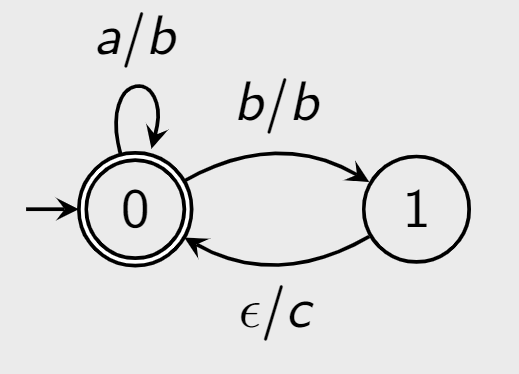
\includegraphics[scale=0.35]{img/cap3/ejemplo1_1.png}
        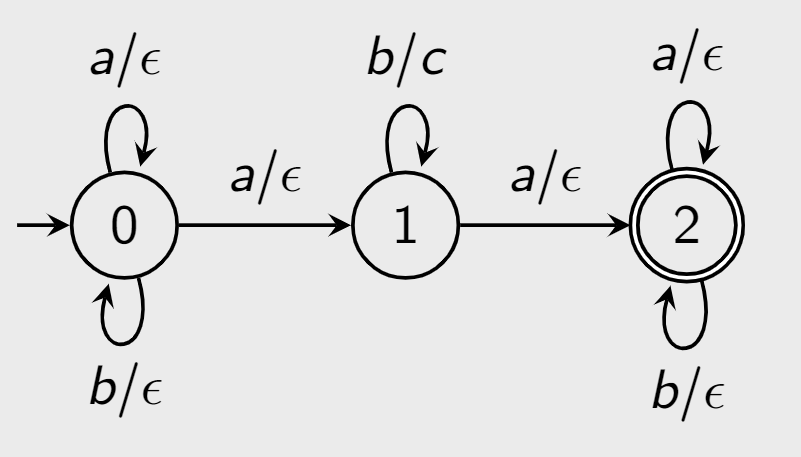
\includegraphics[scale=0.35]{img/cap3/ejemplo1_2.png}
    \end{figure}
}

\paragraph{Configuración.} Sea $\ca{T}$ un transductor. Definimos:
\begin{itemize}
    \item Un par $(q, u, v) \in Q \times \Sigma^* \times \Omega^*$ es una \textbf{configuración} de $\ca{T}$.
    \item Una configuración $(q,u,\epsilon)$ es \textbf{inicial} si $q \in F$.
    \item Una configuración $(q,\epsilon,v)$ es \textbf{final} si $q \in F$.
\end{itemize}

\textit{``Intuitivamente, una configuración $(q, au, vb)$ representa que $\ca{T}$ se encuentra en el estado $q$ procesando la palabra $au$ y leyendo $a$, y hasta ahora grabó la palabra $vb$ y el último símbolo impreso es $b$''.}

\paragraph{Ejecución.} Se define la relación $\vdash_\ca{T}\; \subseteq\left(Q \times \Sigma^* \times \Omega^*\right) \times\left(Q \times \Sigma^* \times \Omega^*\right)$ de \textbf{siguiente-paso} entre configuraciones de $\ca{T}$:
\alignformula{
    \left(p, u_1, v_1\right) \vdash_{\mathcal{T}}\left(q, u_2, v_2\right)
}
si, y sólo si, existe $(p,a,b,q) \in \Delta$ tal que $u_1 = a \cdot u_2$ y $v_2 = v_1 \cdot b$. \medbreak

Se define $\vdash_\ca{T}^*$ como la clausura \textbf{refleja} y \textbf{transitiva} de $\vdash_\ca{T}$:
\alignformula{
    \text{para toda configuración } (q,u,v): \quad &(q, u, v) \vdash_{\mathcal{T}}^*(q, u, v) \\
    \text{si } \left(q_1, u_1, v_1\right) \vdash_{\mathcal{T}}^*\left(q_2, u_2, v_2\right) \text{ y } \left(q_2, u_2, v_2\right) \vdash_{\mathcal{T}}\left(q_3, u_3, v_3\right): \quad &\left(q_1, u_1, v_1\right) \vdash_{\mathcal{T}}^*\left(q_3, u_3, v_3\right)
}
\ejemplo{}{}{
    \vspace{-10pt}
    \img{img/cap3/ejemplo2.png}{0.3}
}

\paragraph{Función definida por un transductor.} Dado un transductor $\ca{T}$, decimos que:
\begin{itemize}
    \item $\ca{T}$ \textbf{entrega} $v$ con \textbf{input} $u$ si existe una configuración inicial $(q_0, u, \epsilon)$ y una configuración final $(q_f, \epsilon, v)$ tal que:
          \alignformula{
              \left(q_0, u, \epsilon\right) \stackrel{\vdash_{\mathcal{T}}^*}{ }\left(q_f, \epsilon, v\right)
          }
    \item Se define la función $\llbracket \mathcal{T} \rrbracket: \Sigma^* \rightarrow 2^{\Omega^*}$:
          \alignformula{
              \llbracket \mathcal{T} \rrbracket(u)=\left\{v \in \Omega^* \mid \mathcal{T} \text { entrega } v \text { con input } u\right\}
          }
    \item Se dice que $f: \Sigma^* \rightarrow 2^{\Omega^*}$ es una \textbf{función racional} si existe un transductor $\ca{T}$ tal que $f=\llbracket \mathcal{T} \rrbracket$.
    \item Un transductor define una función de palabras a conjuntos de palabras.
\end{itemize}

\paragraph{Dos interpretaciones para un transductor.} Podemos ver a $\llbracket \mathcal{T} \rrbracket$ de dos formas:
\begin{enumerate}
    \item $\ca{T}$ define la \textbf{función} $\llbracket \mathcal{T} \rrbracket: \Sigma^* \rightarrow 2^{\Omega^*}$:
          $$
              \llbracket \mathcal{T} \rrbracket(u)=\left\{v \in \Omega^* \mid \mathcal{T} \text { entrega } v \text { con input } u\right\}
          $$
    \item $\ca{T}$ define la \textbf{relación} $\left[\mathcal{T} \rrbracket \subseteq \Sigma^* \times \Omega^*\right.$:
          $$
              (u, v) \in \llbracket \mathcal{T} \rrbracket \quad \text { si, y solo si, } \quad \mathcal{T} \text { entrega } v \text { con input } u
          $$
\end{enumerate}

Desde ahora, hablaremos de función o relación \textbf{indistintamente} y hablaremos de las \textbf{relaciones racionales} (definidas por un transductor).

\paragraph{Lenguaje de input y ouput.} Para una relación $R \subseteq \Sigma^* \times \Omega^*$ se define:
\begin{itemize}
    \item $\pi_1(R)=\left\{u \in \Sigma^* \mid \exists v \in \Omega^* .\ (u, v) \in R\right\}$.
    \item $\pi_2(R)=\left\{v \in \Omega^* \mid \exists u \in \Sigma^* .\ (u, v) \in R\right\}$.
\end{itemize}

\teorema{}{}{
    Si $\ca{T}$ es un transductor, entonces $\pi_1(\llbracket \mathcal{T} \rrbracket)$ y $\pi_2(\llbracket \mathcal{T} \rrbracket)$ son lenguajes regulares sobre $\Sigma$ y $\Omega$, respectivamente.
}

\paragraph{Idea demostración teorema 12.} Para $\ca{T} = (Q,\Sigma,\Omega,\Delta,I,F)$, defina $\ca{A}_1 = (Q, \Sigma, \Delta_1, I, F)$ tal que
$$
    (p, a, q) \in \Delta_1 \quad \text { si, y solo si, } \quad \exists b \in \Omega \cup\{\epsilon\} .\ (p, a, b, q) \in \Delta
$$
y demuestre que $\ca{L}(\ca{A}_1) = \pi_1(\llbracket \mathcal{T} \rrbracket)$.

\teorema{}{}{
    Sea $\ca{T}_1$ y $\ca{T}_2$ dos transductores con $\Sigma$ y $\Omega$ alfabetos de input y output. Las siguientes son \textbf{relaciones racionales}:
    \begin{enumerate}
        \item $$
                  \llbracket \mathcal{T}_1 \rrbracket \cup \llbracket \mathcal{T}_2 \rrbracket=\left\{(u, v) \in \Sigma^* \times \Omega^* \mid(u, v) \in \llbracket \mathcal{T}_1 \rrbracket \vee(u, v) \in \llbracket \mathcal{T}_2 \rrbracket\right\}
              $$
        \item $\llbracket \mathcal{T}_1 \rrbracket \cdot \llbracket \mathcal{T}_2 \rrbracket=\left\{\left(u_1 u_2, v_1 v_2\right) \in \Sigma^* \times \Omega^* \mid\left(u_1, v_1\right) \in \llbracket \mathcal{T}_1 \rrbracket \wedge\left(u_2, v_2\right) \in \llbracket \mathcal{T}_2 \rrbracket\right\}$
        \item $\llbracket \mathcal{T}_1 \rrbracket^*=\bigcup_{k=0}^{\infty} \llbracket \mathcal{T}_1 \rrbracket^k$
    \end{enumerate}
}

La demostración de este teorema queda como ejercicio propuesto al lector.

\teorema{}{}{
    Existen transductores $\ca{T}_1$ y $\ca{T}_2$ sobre $\Sigma$ y $\Omega$ tal que:
    $$
        \llbracket \mathcal{T}_1 \rrbracket \cap \llbracket \mathcal{T}_2 \rrbracket=\left\{(u, v) \in \Sigma^* \times \Omega^* \mid(u, v) \in \llbracket \mathcal{T}_1 \rrbracket \wedge(u, v) \in \llbracket \mathcal{T}_2 \rrbracket\right\}
    $$
    NO es una relación racional.
}
\paragraph{Demostración teorema 14.} Considere los siguientes transductores:
\img{img/cap3/teo14.png}{0.2}
Vemos que $\llbracket \mathcal{T}_1 \rrbracket \cap \llbracket \mathcal{T}_2 \rrbracket=\left\{\left(a^n, b^n c^n\right) \mid n \geq 0\right\}$, pero el lenguaje que define el ouput no es regular, y por lo tanto $\llbracket \mathcal{T}_1 \rrbracket \cap \llbracket \mathcal{T}_2 \rrbracket$ no es racional. \hfill $\blacksquare$

\paragraph{Definición.} Decimos que un transductor $\ca{T}$ define una \textbf{función parcial} si:
\alignformula{
    \text { para todo } u \in \Sigma^* \text { se tiene que }|\llbracket \mathcal{T} \rrbracket(u)| \leq 1 \text {. }
}

\paragraph{Definición.} Decimos que $\ca{T}=(Q,\Sigma,\Omega,\Delta,I,F)$ es \textbf{determinista} si cumple que:
\begin{enumerate}
    \item $\ca{T}$ define una función $\llbracket \mathcal{T} \rrbracket: \Sigma^* \rightarrow \Omega^*$.
    \item para todo $(p,a_1,b_1,q_1)\in\Delta$ y $(p,a_2,b_2,q_2)\in \Delta$, si $a_1=a_2$, entonces
          $$
              b_1=b_2 \quad\text{ y }\quad q_1=q_2
          $$
          Es decir, si tenemos dos transiciones desde un estado $p$ a otros dos estados $q_1$ y $q_2$, y ambas transiciones leen lo mismo: $a_1=a_2$, entonces lo que imprime el transductor y los estados deben ser iguales: $b_1=b_2$ y $q_1=q_2$. Básicamente, buscamos que sean la misma transición.
    \item si $(p,\epsilon,b,q) \in \Delta$, entonces para todo $(p,a',b',q')\in\Delta$, se tiene que
          $$
              (a',b',c')=(\epsilon,b,q)
          $$
          Es decir, si tenemos una $\epsilon$-transición, entonces es la única transición que sale desde $p$.
\end{enumerate}
\ejemplo{}{}{
    \img{img/cap3/ejemplo3.png}{0.35}
}

\subsection{Análisis léxico}

PENDIENTE.

\subsection{Algoritmo de Knuth-Morris-Prat}

\paragraph{Pattern matching.} Veamos el siguiente problema. Dado un \textbf{patrón} $w = w_1 \ldots w_m$ y un documento $d = d_1 \ldots d_n$, encontrar todas las posiciones donde aparece $w$ en $d$, o sea, enumerar:
$$
    \left\{(i, j) \mid w=d_i d_{i+1} \ldots d_j\right\}
$$

Podríamos implementar la siguiente solución ingenua (y poco eficiente):
\vspace{-8pt}
\begin{algorithm}[hbt!]
    % \caption*{An algorithm with caption}\label{alg:two}
    \setstretch{1.25}
    \DontPrintSemicolon
    \SetKw{Output}{output}
    \For{$i=0$ \KwTo $n-m$}{
        $j := 1$

        \While{$j \leq m \wedge w_j = d_{i+j}$}{
            $j := j + 1$
        }

        \If{$j > m$}{
            \Output $(i+1, i+m-1)$
        }
    }
\end{algorithm}
\vspace{-8pt}
\subsubsection{Autómata de un patrón}

\paragraph{Definición.} Dado una palabra $w = w_1 \ldots w_m$, sea el NFA $\ca{A}_w = (Q,\Sigma,\Delta,I, F)$ tal que:
\begin{itemize}
    \item $Q = \{0,1,\ldots,m\}$
    \item $\Delta=\{(0, a, 0) \mid a \in \Sigma\} \cup\left\{\left(i, w_{i+1}, i+1\right) \mid i<m\right\}$
    \item $I = \{0\}$ y $F = \{m\}$.
\end{itemize}
\ejemplo{Palabra $w =$ nano}{}{
    \vspace{-8pt}
    \img{img/cap3/ejemplo4.png}{0.325}
}

Podemos usar $\ca{A}_w$ para encontrar todas las apariciones de $w$ en $w$ haciendo su \textbf{determinización}. \medbreak

\paragraph{Definción.} Sea $\mathcal{A}_w^{\operatorname{det}}=\left(Q^{\operatorname{det}}, \Sigma, \delta^{\operatorname{det}},\{0\}, F^{\operatorname{det}}\right)$ la determinización de $\ca{A}_w$ tal que $Q^\text{det}$ contiene \textbf{solo los estados alcanzables} desde $\{0\}$.

\ejemplo{Palabra $w =$ nano y $d =$ un nano no nana}{}{\
    \vspace{-8pt}
    \img{img/cap3/ejemplo5.png}{0.325}
    $$
        \begin{array}{ccccccccccccccccccc}
            q_0 & q_0 & q_1 & q_0 & q_1 & q_2 & q_3 \checkmark & q_4 & q_0 & q_1 & q_0 & q_0 & q_1 & q_2 & q_3 & q_2 \\
            u   & n   &     & n   & a   & n   & o              &     & n   & o   &     & n   & a   & n   & a         \\
            1   & 2   & 3   & 4   & 5   & 6   & 7              & 8   & 9   & 10  & 11  & 12  & 13  & 14  & 15
        \end{array}
    $$
}

\teorema{}{}{
    Para todo $S \in Q^\text{det}$ y $i \in \{0,1,\ldots,m\}$ se cumple que
    $$
        i \in S \quad \text { si, y solo si, } \quad w_1 \ldots w_i \text { es un sufijo de } w_1 \ldots w_{\max (S)} \text {. }
    $$
}

\paragraph{Corolarios.} Tenemos que:
\begin{itemize}
    \item Para todo $S_1,S_2 \in Q^\text{det}$, si $\max(S_1) = \max(S_2)$, entonces $S_1 = S_2$.
    \item $\ca{A}_w^\text{det}$ tiene $|w| + 1$ estados y a lo más $\ca{O}(|w|^2)$ transiciones.
\end{itemize}

Por lo tanto, encontrar todos los substrings de $w$ en $d$ toma tiempo $\ca{O}(|d| + |w|^2)$.

\paragraph{Demostración teorema 15.} Sea $S \in Q^\text{det}$ un conjunto de estados cualquiera alcanzable desde $\{0\}$. Entonces, existe una palabra $u = a_1 \ldots a_k$ tal que $\hat{\delta}^{\operatorname{det}}(\{0\}, u)=S$. Por la demostración de que $\mathcal{L}\left(\mathcal{A}^{\mathrm{det}}\right)=\mathcal{L}(\mathcal{A})$ para todo NFA $\ca{A}$, sabemos que $j \in S$ si, y sólo si, existe una ejecución $\ca{A}_w$ sobre $u$:
$$
    0=q_0 \stackrel{a_1}{\rightarrow} q_1 \stackrel{a_2}{\rightarrow} \ldots \stackrel{a_k}{\rightarrow} q_k=j
$$
Por la definición de $\ca{A}_w$ esta ejecución es de la forma:
$$
    0 \stackrel{a_1}{\rightarrow} 0 \stackrel{a_2}{\rightarrow} \ldots \stackrel{a_{k-j}}{\rightarrow} 0 \underbrace{\stackrel{a_{k-j+1}}{\rightarrow} 1 \stackrel{a_{k-j+2}}{\rightarrow} 2 \ldots \stackrel{a_k}{\rightarrow}}_{w_1 \ldots w_j} j
$$
Por lo tanto, $w_1 w_2 \ldots w_j$ es sufijo de $a_1 \ldots a_k$. Usaremos este último hecho para demostrar \textbf{ambas} direcciones del teorema, que formalizamos a continuación. \medbreak

\textit{Propiedad.} Para toda $u = a_1\ldots a_k$ tal que $\hat{\delta}^{\operatorname{det}}(\{0\}, u)=S$, y para todo $j \leq m$:
$$
    j \in S \quad \text { si, y solo si, } \quad w_1 \ldots w_j \text { es sufijo de } a_1 \ldots a_k
$$

\textit{Demostración $(\Rightarrow)$.} Como $S$ es alcanzable desde $\{0\}$, entonces existe $u = a_1 \ldots a_k$ tal que $\hat{\delta}^{\operatorname{det}}(\{0\}, u)=S$. Como $\max(S) \in S$, entonces $W_1 \ldots W_{\max }(S)$ es sufijo de $a_1 \ldots a_k$. \medbreak

Suponga que $i \in S$. Entonces $w_1 \ldots w_i$ es sufijo de $a_1 \ldots a_k$. Como $i \leq \max(S)$, entonces:
$$
    a_1 a_2 \ldots a_{k-\max(S)} \overbrace{a_{k-\max(S)+1} \ldots a_{k-i} \underbrace{a_{k-i+1}\ldots a_k}_{w_1\ldots w_i}}^{w_1\ldots w_{\max(S)}}
$$
Por lo tanto, $w_1 \ldots w_i$ es sufijo de $w_1 \ldots w_{\max(S)}$. \medbreak

\textit{Demostración $(\Leftarrow)$.} Como $S$ es alcanzable desde $\{0\}$, entonces existe $u = a_1 \ldots a_k$ tal que $\hat{\delta}^{\mathrm{det}}(\{0\}, u)=S$. Como $\max(S) \in S$, entonces $w_1 \ldots w_{\max(S)}$ es sufijo de $a_1 \ldots a_k$. \medbreak

Suponga que $w_1 \ldots w_i$ es sufijo de $w_1 \ldots w_{\max(S)}$. Como $w_1 \ldots w_i$ es sufijo de $w_1 \ldots w_{\max(S)}$ y $w_1 \ldots w_{\max(S)}$ es sufijo de $u$, entonces $w_1 \ldots w_i$ es sufijo de $u = a_1 \ldots a_k$. \medbreak

Por la ``propiedad'', concluimos que $i \in S$. \hfill $\blacksquare$

\subsubsection[Autómata finito con k-lookahead]{Autómata finito con $k$-lookahead}

\paragraph{Definición}. Se definen los siguientes conjuntos de palabras sobre un alfabeto finito $\Sigma$:
\begin{itemize}
    \item $\Sigma_{\bullet}=\Sigma^* \times \Sigma^*$
    \item $\Sigma_{\bullet}^k=\left\{(u, v) \in \Sigma_{\bullet}\mid |uv| = k\right\}$
\end{itemize}

\paragraph{Notación.} En vez de $(u,v) \in \Sigma_\bullet$, escribiremos $u.v \in \Sigma_\bullet$.

\ejemplo{}{}{
    Si $\Sigma = \{a,b\}$, entonces:
    \begin{itemize}
        \item $ab.ba \in \Sigma_\bullet$ y $.aba \in \Sigma_\bullet$
        \item $ab.ba \in \Sigma_\bullet^4$ y $.aba \in \Sigma_\bullet^3$
    \end{itemize}
}

\paragraph{Definición.} Un autómata finito determinista con $k$-lookahead es una tupla:
\alignformula{
    \ca{A} = (Q, \Sigma, \delta, q_0, F)
}
\begin{itemize}
    \item $Q$ es un conjunto finito de estados.
    \item $\Sigma$ es el alfabeto del input.
    \item $q_0$ es el estado inicial.
    \item $F \subseteq Q$ es el conjunto de estados iniciales.
    \item $\delta: Q \times(\Sigma \cup\{\mathbb{\$}\})_{\bullet}^k \rightarrow Q$ es una función parcial, tal que:
          $$
              \text { para todo } p \in Q \text { y } w \in(\Sigma \cup\{\$\})^k:\quad  |\{u . v \mid \delta(p, u \cdot v)=q \text { y } u v=w\}| \leq 1
          $$
\end{itemize}
\ejemplo{}{}{
    \begin{figure}[H]
        \centering
        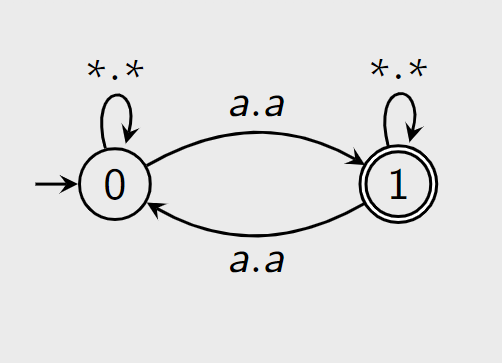
\includegraphics[scale=0.4]{img/cap3/ejemplo6_1.png}
        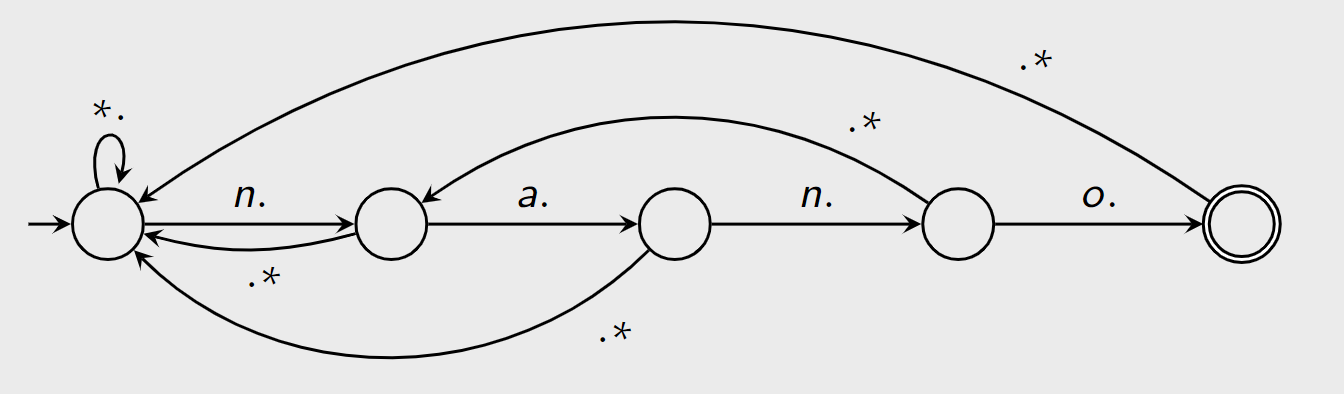
\includegraphics[scale=0.4]{img/cap3/ejemplo6_2.png}
    \end{figure}
}

\paragraph{Ejecución.} Sea $\ca{A}$ un DFA con $k$-lookahead. Tenemos que:
\begin{itemize}
    \item Un par $(q, w) \in Q \times(\Sigma \cup\{\$\})^*$ es una \textbf{configuración} de $\ca{A}$.
    \item Una configuración $(q_0, w\$^k)$ es \textbf{inicial}.
    \item Una configuración $(q, \$^k)$ es \textbf{final} si $q \in F$.
\end{itemize}

El sufijo $\$^k$ nos sirve para marcar el finald el input (y simplificar la definición de lookahead al leer el final de la palabra). \medbreak

Se define la relación $\vdash_\ca{A}$ de \textbf{siguiente-paso} entre configuraciones de $\ca{A}$:
\alignformula{
    \left(p_1, w_1\right) \vdash_\mathcal{A}\left(p_2, w_2\right)
}
si, y sólo si, $\delta\left(p_1, u . v\right)=p_2$ y existe $w \in \Sigma^*$ tal que $w_1 = uvw$ y $w_2 = vw$. \medbreak

Se define $\vdash_\ca{A}^*$ como la clausura \textbf{refleja} y transitiva de $\vdash_A$:
\alignformula{
    \text{para toda configuración } (p,w): \quad &(p,w) \vdash_\ca{A}^* (p,w) \\
    \text{si } (p_1, w_1) \vdash_\ca{A}^* \text{ y } (p2,w_2) \vdash_\ca{A} (p_3,w_3): \quad &\left(p_1, w_1\right) \vdash_{\mathcal{A}}^*\left(p_3, w_3\right)
}

Decimos que $(p,u) \vdash_\ca{A}^* (q,v)$ si uno puede ir de $(p,u)$ a $(q,v)$ en \textbf{0 o más pasos}.

\paragraph{Aceptación.} Decimos que $\ca{A}$ \textbf{acepta} $w$ si existe una configuración inicial $(q_0, w\$^k)$ y una configuración final $(q_f, \$^k)$ tal que:
$$
    \left(q_0, w \mathbb{S}^k\right) \vdash_{\mathcal{A}}^*\left(q_f, \mathbb{S}^k\right)
$$
El \textbf{lenguaje aceptado} por $\ca{A}$ se define como:
$$
    \mathcal{L}(\mathcal{A})=\left\{w \in \Sigma^* \mid \mathcal{A} \text { acepta } w\right\}
$$
Vemos que son las mismas definiciones para un $\epsilon$-NFA.

\teorema{}{}{
    Para todo DFA con $k$-lookahead $\ca{A}$ se tiene que $\ca{L}(\ca{A})$ es un \textbf{lenguaje regular}.
}
La demostración de este teorema queda como ejercicio propuesto al lector.

\paragraph{Definición.} Llamaremos un \textbf{lazy autómata} a un DFA con $1$-lookahead.

\subsubsection{Algoritmo KMP}

\paragraph{Construcción de un lazy automata.} Sea $w = w_1 \ldots w_m$ y $\mathcal{A}_w^{\mathrm{det}}=\left(Q^{\mathrm{det}}, \Sigma, \delta^{\mathrm{det}},\{0\}, F^{\mathrm{det}}\right)$ la determinización de $\ca{A}_w$.

\paragraph{Definición.} Para $i \in [0,m]$, sea $S_i$ el \textbf{único estado} en $Q^\text{det}$ tal que $i = \max(S_i)$.

\paragraph{Propiedad.} Para todo $a \in \{w_1,\ldots w_m\}$ y $i \in [0,m-1]$:
\begin{enumerate}
    \item $S_i-\{i\} \in Q^{\operatorname{det}}$
    \item $a=w_{i+1}$, entonces $\delta^{\operatorname{det}}\left(S_i, a\right)=S_{i+1}$.
    \item $a \neq w_{i+1}$, entonces $\delta^{\operatorname{det}}\left(S_i, a\right)=\delta^{\operatorname{det}}\left(S_i-\{i\}, a\right)$.
\end{enumerate}
La demostración de esta propiedad queda como ejercicio propuesto al lector. \medbreak

En base a la propiedad anterior, se define el lazy autómata $\mathcal{A}_w^{\text {lazy}}=\left(Q^{\text {det}}, \Sigma, \delta^{\text {lazy }},\{0\}, F^{\text {det }}\right)$ tal que:
\begin{itemize}
    \item para todo $a\neq w_1$: $\delta^{\text {lazy}}(\{0\}, a .)=\{0\}$.
    \item para todo $a \in \{w_1,\ldots, w_m\}$ y $i \in [0,m-1]$:
          \begin{itemize}
              \item si $a = w_{i_1}$, entonces $\delta^{\text {lazy}}\left(S_i, a_{.}\right)=S_{i+1}$
              \item si $a \neq w_{i+1}$ y $i \neq 0$, entonces $\delta^{\text {lazy}}\left(S_i, . a\right)=S_i-\{i\}$.
          \end{itemize}
\end{itemize}
\ejemplo{}{}{
    \img{img/cap3/ejemplo7.png}{0.35}
}

\teorema{}{}{
    Para todo $w$ se cumple que $\mathcal{L}\left(\mathcal{A}_w^{\text {det}}\right)=\mathcal{L}\left(\mathcal{A}_w^{\text {lazy}}\right)$.
}
La demostración queda como ejercicio propuesto para el lector (usando la propiedad).

\paragraph{Complejidad KMP.} Vemos que:
\begin{itemize}
    \item El número de pasos que $\ca{A}_w^\text{lazy}$ \textbf{consume} letras $= |d|$
    \item El número de pasos que $\ca{A}_w^\text{lazy}$ \textbf{retrocede} $\leq |d|$
    \item El número de \textbf{pasos totales} de $\ca{A}_w^\text{lazy}$ $\leq 2 \cdot |d|$
\end{itemize}
Por lo tanto, la cantidad de pasos es \textbf{lineal} en $\ca{O}(|d|)$.

\paragraph{Algoritmo KMP.} Dado una palabra $w$ y un documento $d$:
\begin{enumerate}
    \item Construimos $\ca{A}_w^\text{lazy}$ desde $\ca{A}_w$.
    \item Ejecutamos $\ca{A}_w^\text{lazy}$ sobre $d$.
\end{enumerate}

El paso 1 toma $\ca{O}(|w|)$ y el paso 2 toma $\ca{O}(|d|)$, por lo tanto, el tiempo del algoritmo es $\ca{O}(|w| + |d|)$. \medbreak

Queda como ejercicio para el lector demostrar que construir $\ca{A}_w^\text{lazy}$ toma tiempo $\ca{O}(|w|)$.




